\chapter*{Chiloe : journée à Puñihuil\markboth{Chiloe : journée à Puñihuil}{}}
\section*{18 février 2015}
Enfin une journée qui s'annonce sous le soleil !
\begin{center} 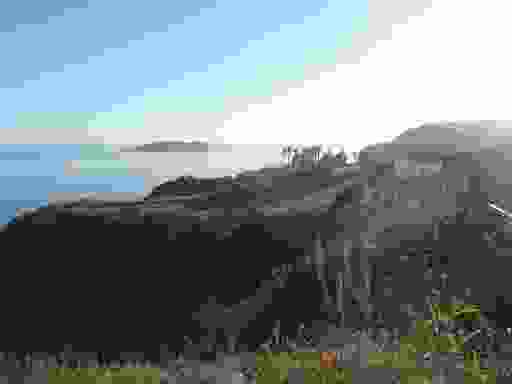
\includegraphics[width=\mywidth]{../wp-content/uploads/2015/02/P2122067.jpg} \end{center}

\pagebreak
 30km de belle route le long de la côte pour aller à la Pinguineria de Puñihuil.
\begin{center} 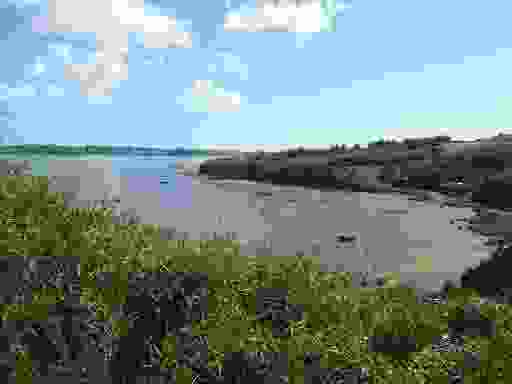
\includegraphics[width=\mywidth]{../wp-content/uploads/2015/02/P2122070.jpg} \end{center}
\begin{center} 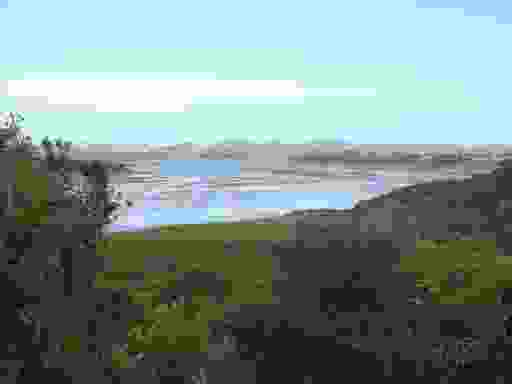
\includegraphics[width=\mywidth]{../wp-content/uploads/2015/02/P2122072.jpg} \end{center}
\begin{center} 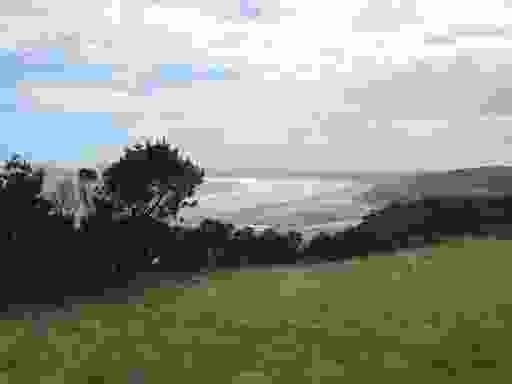
\includegraphics[width=\mywidth]{../wp-content/uploads/2015/02/P2122073.jpg} \end{center}
\begin{center} 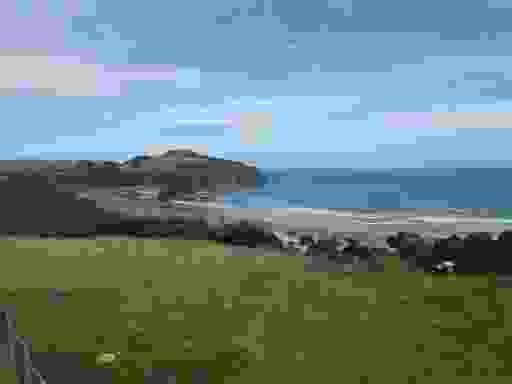
\includegraphics[width=\mywidth]{../wp-content/uploads/2015/02/P2122074.jpg} \end{center}
\begin{center} 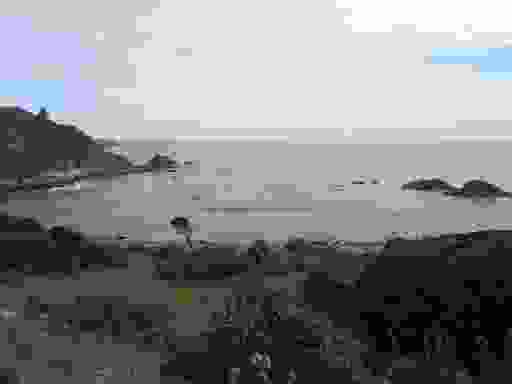
\includegraphics[width=\mywidth]{../wp-content/uploads/2015/02/P2122075.jpg} \end{center}

 Rencontre avec Carlo, un cycliste italien :
\begin{center} 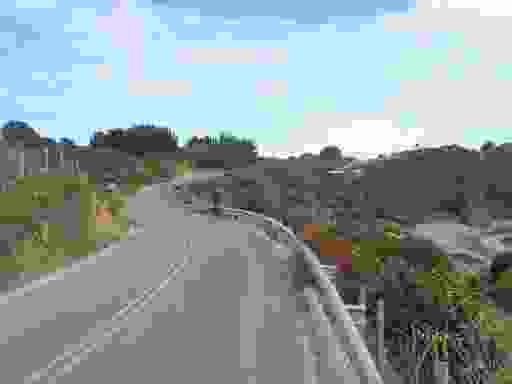
\includegraphics[width=\mywidth]{../wp-content/uploads/2015/02/P2122077.jpg} \end{center}

\pagebreak
 Tour en bateau depuis la plage :
\begin{center} 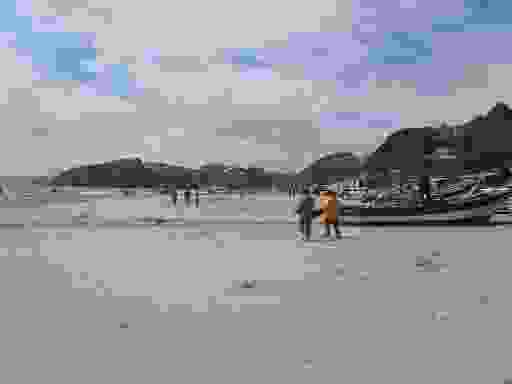
\includegraphics[width=\mywidth]{../wp-content/uploads/2015/02/P2122079.jpg} \end{center}
\begin{center} 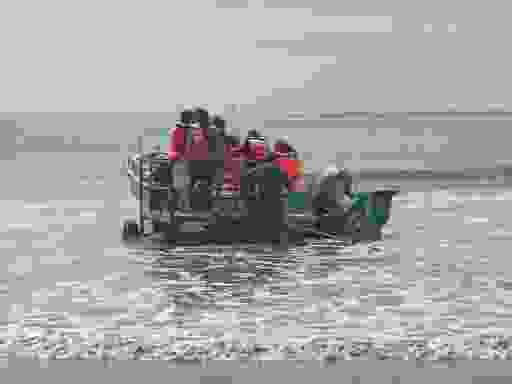
\includegraphics[width=\mywidth]{../wp-content/uploads/2015/02/P2122080.jpg} \end{center}

\pagebreak
 Il y a 2 espèces différentes de pingouins sur l'île. 
\begin{center} 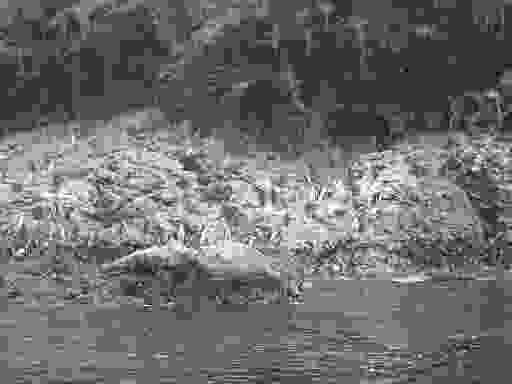
\includegraphics[width=\mywidth]{../wp-content/uploads/2015/02/P2122084.jpg} \end{center}
\begin{center} 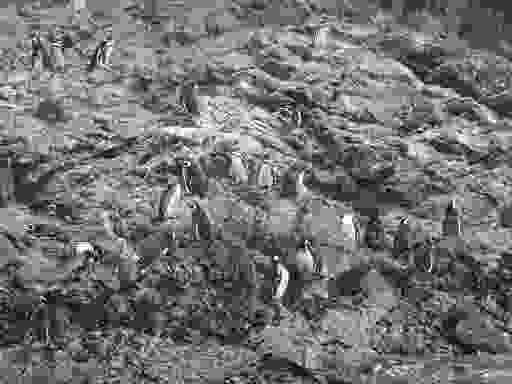
\includegraphics[width=\mywidth]{../wp-content/uploads/2015/02/P2122087.jpg} \end{center}
\begin{center} 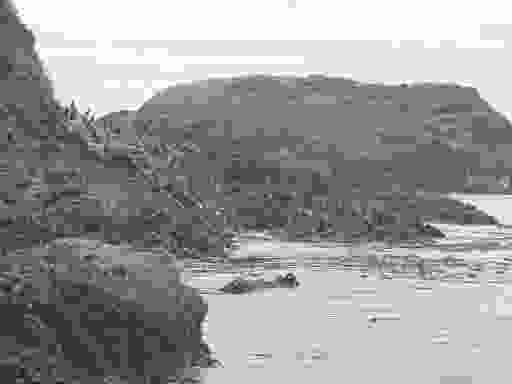
\includegraphics[width=\mywidth]{../wp-content/uploads/2015/02/P2122088.jpg} \end{center}

 Des pélicans :
\begin{center} 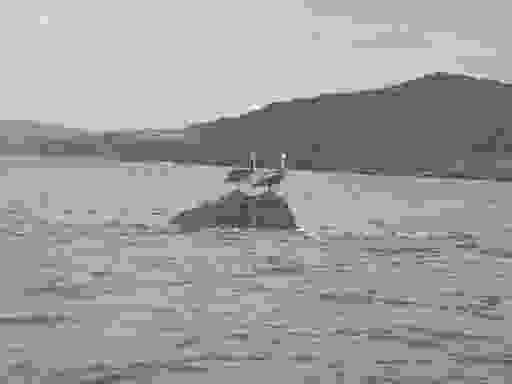
\includegraphics[width=\mywidth]{../wp-content/uploads/2015/02/P2122094.jpg} \end{center}

 Je reprend la route avec Carlo sur un chemin en gravier qui enchaîne montées et descentes raides. 
 Trop difficile pour mon vélo : le filetage qui fixe les pignons au moyeu est mort et je ne peux plus avancer car je pédale dans le vide.
\begin{center} 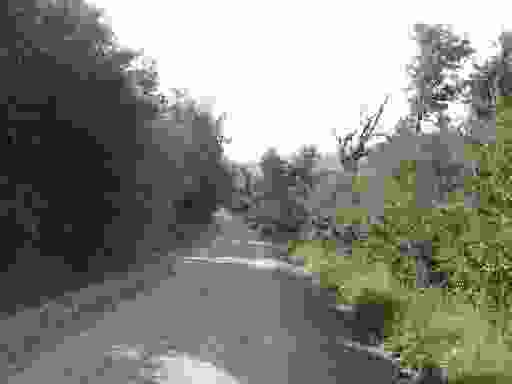
\includegraphics[width=\mywidth]{../wp-content/uploads/2015/02/P2122095.jpg} \end{center}

 Demi-tour pour rejoindre la route à pied : par chance un pick-up s'arrête et accepte de me déposer à Ancud.
 Changement du moyeu dans un magasin de vélos, le technicien est efficace il a démonté, remonté tous les rayons de la roue arrière et dévoilé la roue en à peine 1h et demie.

 Du coup je retourne au même camping que la veille et je recroise Javier et Jonathan, 2 voyageurs à vélo que j'avais déjà rencontrés.
\begin{center} 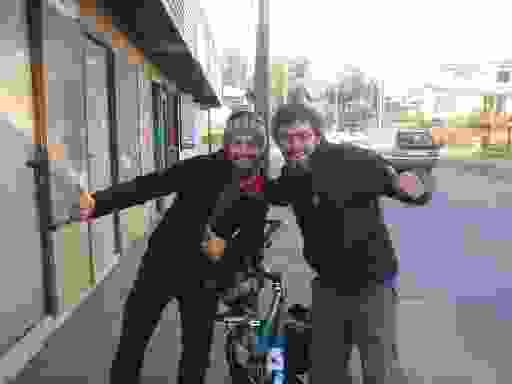
\includegraphics[width=\mywidth]{../wp-content/uploads/2015/02/P2132096.jpg} \end{center}